\documentclass[final,5p,12pt,twocolumn]{elsaarticle}
\usepackage{amssymb}
\usepackage{amsmath}
\usepackage{multicol}
\usepackage{graphicx}
\usepackage{svg}
\newcommand{\kms}{km\,s$^{-1}$}
\newcommand{\msun}{$M_\odot}
\usepackage{blindtext}
\usepackage{titlesec}
\graphicspath{ {./images/} }
\usepackage{blindtext}
\usepackage{minted}
\usepackage{fancyvrb}
\usepackage{subfigure}


\begin{document}
%% \title{Comprehensive analysis of electronic noise and their noise spectra of zener diode}
%% \author{Vijay Panchal}
%% \author{Ved Rudani}
%% \address{Department of Physics, Electronics and Space Sciences, Gujarat University, Ahmedabad, India}



\parbox[h]{.8\textwidth}{\centering \vskip-20pt
\parbox[h]{.75\textwidth}{\centering
\includegraphics[width=300pt]{GUlogo.pdf}}
%%     \vskip50pt
    \parbox[b]{.75\textwidth}{\centering\Huge Project Report \par}\vskip10pt
    \parbox[b]{.75\textwidth}{\centering\hrule height 2pt \vskip30pt\Huge\textbf{Comprehensive analysis of electronic noise and their noise spectra of voltage regulator circuit with zener diode at low frequency}\par}\vskip20pt
   \parbox[b]{.75\textwidth}{\centering \LARGE MSc Semester $3$}\vskip7pt
    \parbox[b]{.75\textwidth}{\centering \large Unit 505:  Project Work}\vskip20pt 
%%    \parbox[b]{.75\textwidth}{\centering\normalsize\elsauthors\par}\vskip10pt

    \parbox[b]{.75\textwidth}{\centering\normalsize \textbf{\emph{Ved Rudani}}   Roll number: \textbf{54}\par}\vskip2pt
    \parbox[b]{.75\textwidth}{\centering\normalsize \textbf{\emph{Vijay Panchal}}  Roll number: \textbf{55}\par}\vskip25pt
%%     \parbox[b]{.75\textwidth}{\centering\footnotesize\itshape\elsaddress\par }

 \parbox[b]{.75\textwidth}{\centering\normalsize Under the the guidance of: }\vskip10pt

 \parbox[b]{.75\textwidth}{\centering\normalsize \Large \textbf{D. B. Patel}}\vskip10pt
 \parbox[b]{.75\textwidth}{\centering\normalsize \Large \textbf{U. S. Joshi}}\vskip10pt
 \parbox[b]{.75\textwidth}{\centering\normalsize Department of Physics, Electronics and Space Sciences, Gujarat University, Ahmedabad,380009}\vskip10pt
 \vskip20pt\hrule height 2pt
}

\begin{table*}[hbt!]\centering
  %% \vskip0pt
  \parbox[h]{.75\textwidth}{\centering \hrule height 2pt \vskip10pt\Large \textbf{Abstract} \vskip10pt \hrule height 2pt \vskip10pt}
  \parbox[h]{.75\textwidth}{\normalsize \textbf{
       We present a noise analysis of regulated power supplies. Basic zener diode regulated power supply is employed. We studied noise characteristics at very low frequency (sub hertz), low frequency(up to 10k) and relatively high frequency (up to 100k). All this analysis is made from the LOCK IN amplifier which gives us direct frequency domain information about the device. For our purpose we used SR830 which is relatively low noise compared to our noise signal and can measure up to 10nV/Hz. We looked for traces of frequency dependent noise like flicker noise and  white noise like shot noise, avalanche noise and thermal noise. We used a specific \emph{zener diode} specifically BZX55C5V1 in the voltage regulator, which means exact results can be varied to different zener diodes but it should follow a similar trend. Our work in interfacing with the LOCK IN amplifier led to a new python package called \emph{pyinstro}, which was intended as stream lined for laboratory instrument controlling and handling. We tried to make it as flexible and extensible as possible. This library is made as open source and supports every SCPI supported interface like GPIB, RS232, USB and LAN.  This project is done as our semester project. 
} \vskip10pt \hrule height 2pt \vskip10pt}
\end{table*}
\clearpage
\begin{table*}[hbt!]\centering
\vskip100pt
\parbox[h]{.75\textwidth}{\tableofcontents}
\end{table*}
\clearpage


\section{Introduction}\label{introduction}

Regulated power sources are extremely important in day to day lab work. Zener diodes and passive elements share an integral part of the overall circuit of regulated power supply.  When we are dealing with precision measurement and study we need the most precise power sources to work with but because of 'Noise' of components of zener diodes and passive elements it inherits noise internally. Since, this noise will be infested in precision work we are doing in the lab. It is better to study the known structure of noise in these devices to address methodic treatment to our data and circuits. With all this in mind we are doing noise measurement and studying the noise spectrum of the zener diode.

For this semester we had radical plans to try but it evolved into more mature or downgraded in a way. First tried as shot noise to generate a random number generator which could possibly be a true random generator with little transformations. Then we eyed the more on general idea of studying noise theoretically and doing analysis experimentally. Which is exactly what we are doing right now but change is that at start we are working with photodiode and now with zener diode. Thanks to Dr. U S Joshi sir who guided us to try different diodes against photodiode. In this report we are having the following parts in order. First we are studying theoretically components, then we will discuss methods and tools that we used included all instrumentation, data acquisition, data analysis etc., we will conclude with our results and discuss it. The foundational work in thermal noise was done by J B johnson in his paper [site it]. 




\section{Theoretical compilation}\label{Theory}

This section will deal with theoretical components from our project. Here, linear circuit analysis gives noise and output voltage relationship. 

\subsection{Linear circuit analysis \label{lca}}


We have a voltage regulator circuit from a zener diode which regulates voltages at specific voltage known as zener voltage $V_{z}$. The fluctuation from these regulated voltages is what we call noise. Since ideal regulators only give pure DC voltages at output, this fluctuation is completely unwanted and only be resultant of intrinsic noise of this regulator circuit.  We limit ourselves with only noise coming from zener diode which is not quite good practice. Since, noise can be added from extra resistors, wires and even the power supply itself. The resistor noise can be neglected because of their low values as we used 10k in series and 100k in parallel to output. We will see this later.

Let’s take a basic voltage regulator circuit as shown in figure \ref{thcir1}.

\begin{figure}[hbt!]
\centering{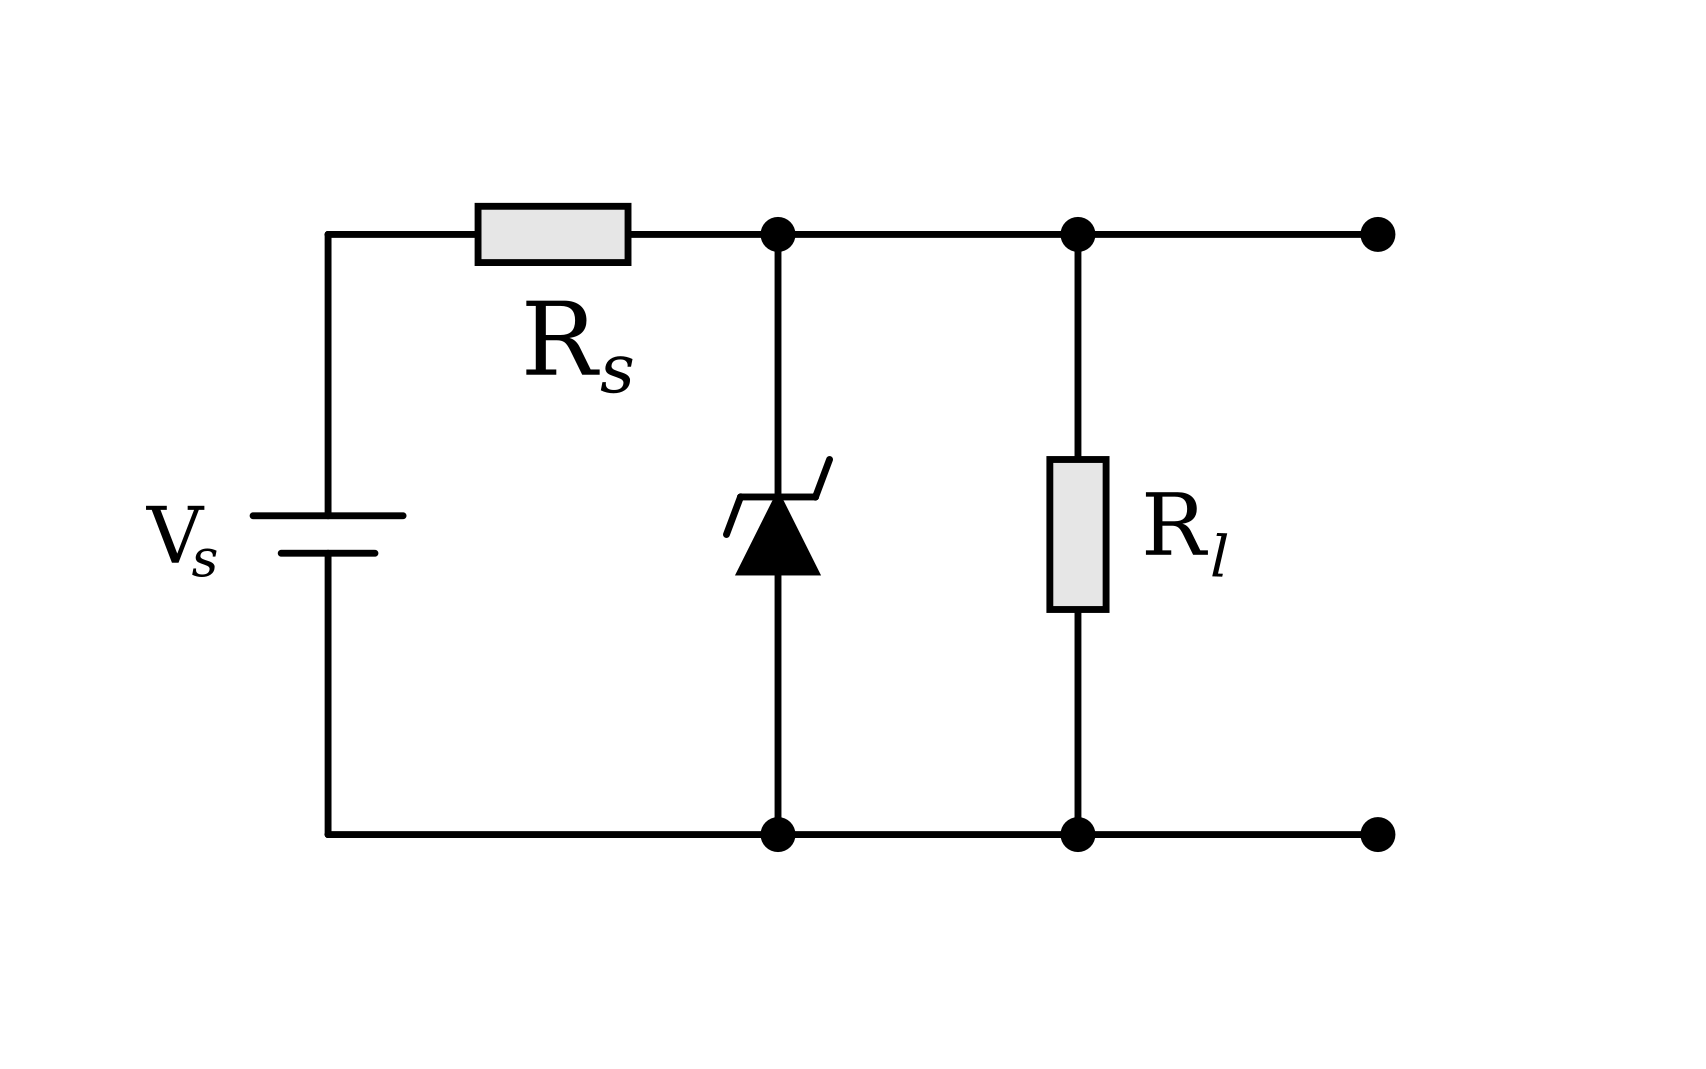
\includegraphics{circuit-20231005-2243.png}}
\caption{Simple voltage regulator circuit made from zener diode \label{thcir1}}
\end{figure}

As you can see we have a zener diode parallel to the power supply, which regulates at a certain degree. Since this is a linear circuit output voltage can be easily derived.

Applying kirchhoff current low in the figure \ref{thcir1},


\begin{align*}
I_{z} & = I_{R_s} -I_{L}\\
& = \frac{V_s-V_o}{R_s}-\frac{V_o}{R_L}\\
& = -V_o(\frac{1}{R_s}+\frac{1}{R_L})+ \frac{V_s}{R_s}
& = -V_oA^{\prime}+B^{\prime}
\end{align*}

Here, $A^{\prime} = \frac{1}{R_s}+\frac{1}{R_L})$ and $B^{\prime} = \frac{V_s}{R_s}
$.  

We can write $I_z = \frac{V_z}{R_z}$, where $V_z$ and $R_z$ are respectively zener voltages and impedance.  This relation is quite linear in the breakdown region as you can see in the figure \ref{thiv}. \footnote{Image is taken from Electronics Devices and Circuit Theory by Robert Boylsted}

\begin{figure}[hbt!]
\centering{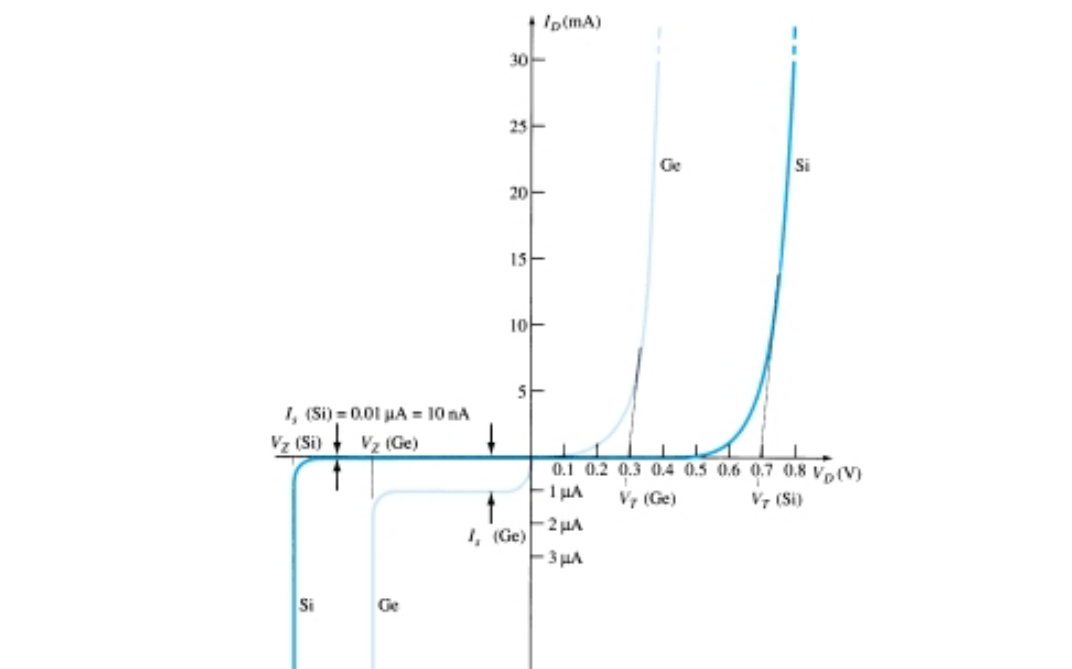
\includegraphics[width=350pt]{thzenerIV.png}}
\caption{theoretical current and voltage relation for zener diode \label{thiv}}
\end{figure}


Here we can assume equivalent circuit of \ref{thecir1} as figure \ref{thcir} 

\begin{figure}[hbt!]
\centering{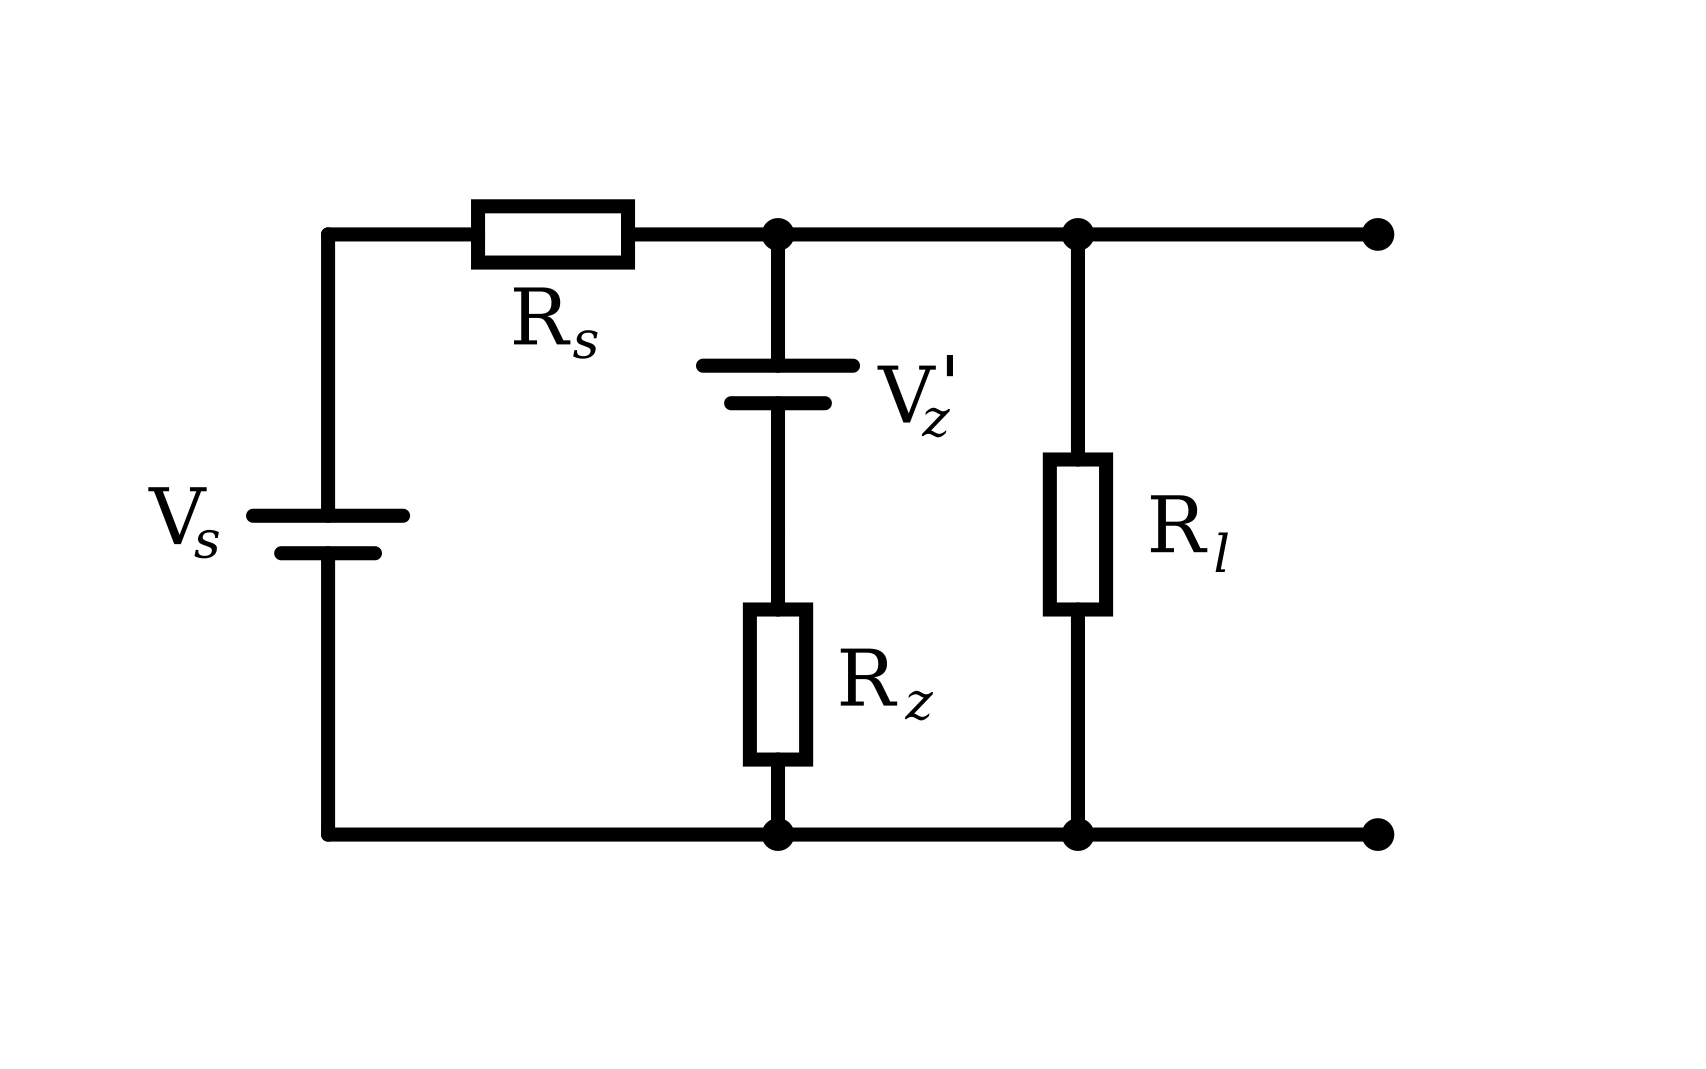
\includegraphics{circuit-20231005-2244.png}}
\caption{Equivalent circuit of figure \ref{thcir1} \label{thcir2}}
\end{figure}

Further, simplifying the circuit,

\begin{figure}[hbt!]
\centering{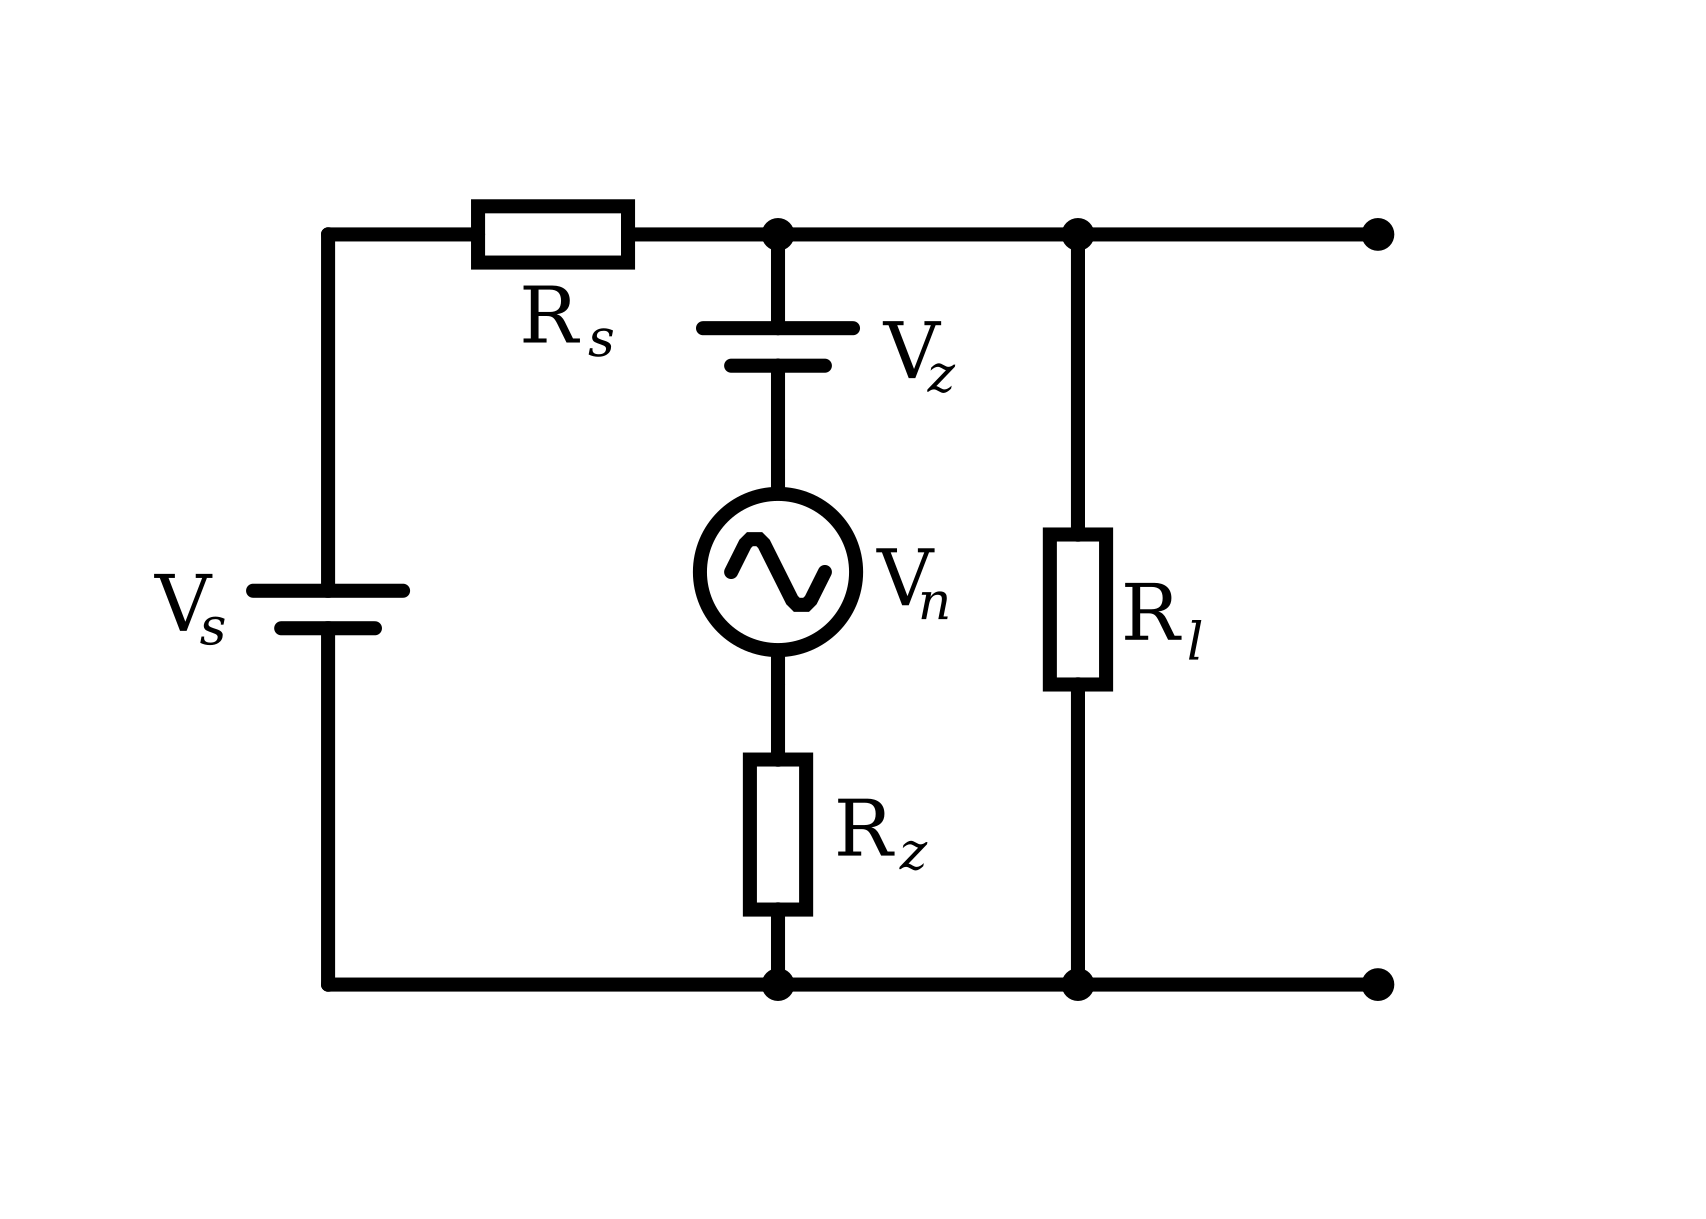
\includegraphics{circuit-20231005-2245.png}}
\caption{Equivalent circuit of figure \ref{thcir2} \label{thcir3}}
\end{figure}

This circuit is further simplified as we take $V_z = V_{DC} + V_n$ where $V_n$ is the noise voltage of the zener diode.
If we neglect noise from other sources like resistors and power supply then from figure \ref{thcir3},

\begin{align*}
\frac{V_z}{I_z} & = -V_oA^{\prime} +B^{\prime}\\
  \\
\frac{V_{DC}+V_n}{I_z} & =  -V_oA^{\prime} +B^{\prime}\\
\\  
V_n & = -V_oA+B
\end{align*}


\begin{align} \label{vo}
V_o & = -\frac{V_n}{A}+\frac{B}{A}
\end{align}



So, we can conclude that here as $V_o \propo V_n$.  This will be the main focus of this project. Here we are neglecting $V_{DC}$ and will be totally okay when we read data from the LOCK IN amplifier, since the DC component has zero frequency which can’t be read from the LOCK IN amplifier.

\subsection{Different noises in the circuit \label{thno}}

The noise voltage $V_n$ is made from different types of noise source which can act as a symbol voltage source. So, $V_n$ can be broken into sub noise sources such as $V_n = V_{flicker}+V_{thermal} + V_{shot} +\cdots$. We will see this noise source and its origin then we will derive its respective distribution and equations.

\begin{figure}[hbt!]
\centering{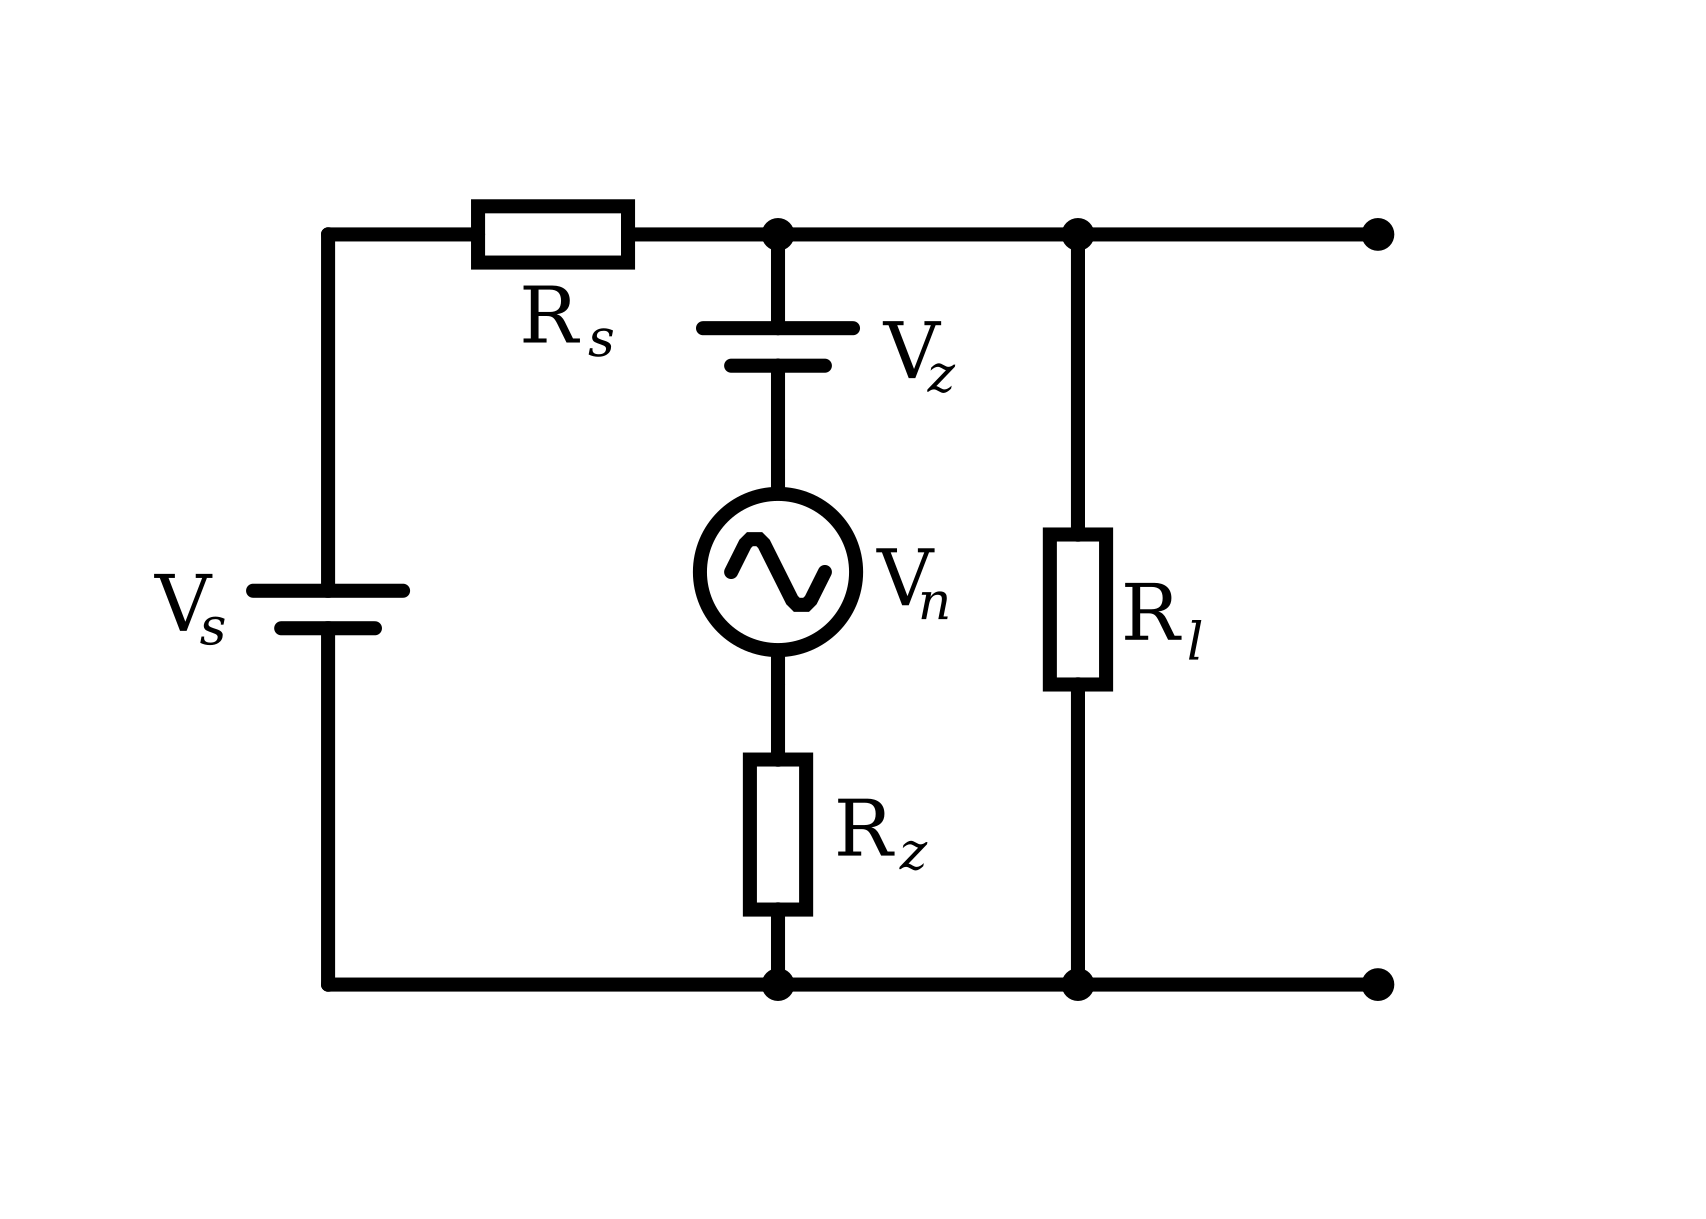
\includegraphics{circuit-20231005-2245.png}}
\caption{Equivalent noise sources \ref{thcir2} \label{thcir4}}
\end{figure}

\subsubsection{Flicker Noise \label{thflicker}}

Flicker noise is also known as 1/f noise in view of the fact that power density decreases with increasing frequency. This implies that at lower frequencies, the flicker noise dominates.
This type of noise is found  almost in any electronic device which is able to operate at lower frequencies.The main source of this type of noise is D.C supply. Its first evidence was given by J. B. Johnson \cite{j b johnson}. Its first 1/f form is derived by beck and spruit \cite{beck and spruit}. Now the form is given as 

\begin{align}
S(f) & = \frac{C}{f^{\alpha}}
\end{align}

Here, $C$ and $\alpha$ determine the nature of flicker noise. $\alpha determine relations with other noise elements$.

\begin{enumerate}
\item ($\alpha > 0$): This means that white noise is dominating the flicker noise as frequency increases.
\item ($\alpha = 0$): This means that only white noise is exists
\item ($\alpha < 0$): This means noise is increasing as frequency. Also, shows that noise will be persistent with a higher range of frequencies. Typically white noise dominates traditional flicker noise.
\end{enumerate}

We can see noise levels as from figure \ref{thnoise}.

\subsubsection{Shot noise \label{thshot}}

Shot noise is a form of noise that arises because of the discrete nature of the charges carried by charge carriers, electrons or holes or photons hitting the surface. Shot noise is analogous to the rainfall in which raindrop hitting the surface can be considered as discrete. The sound of rainfall is very similar to noise we hear from speakers when we are considering shot noise. 

Since, shot noise is a phenomenon for discrete charge passing through a junction, it can be modelled by poisson distribution. Suppose that In the time interval the $\tau$ Q charge passes through a junction in a semiconductor device (in present context zener diode). This gives rise to discrete probability distribution,

\begin{align}
P(N) & = \frac{e^{-\lambda \tau}(\lambda \tau)^{N}}{N!}
\end{align}

If $N=0$ charge passes in time interval $\tau$ then $P(N)$will be,

\begin{align} \label{eqN0}
P(0) & = e^{-\lambda \tau}
\end{align}

Now suppose, probability of one and only one charge passing through junction in time $\tau$,

\begin{align*}
P(\tau)d\tau & = (P_{\tau}(0))(P_{\tau}(1))
\end{align*}

From equation \ref{thN0},


\begin{align*}
P(\tau)d\tau & = (e^{-I_0 \tau})(e^{-I_0 d\tau} I_0 d\tau)\\
\\  
P(\tau) & = (e^{-I_0 (\tau + d\tau)}) I_0
\end{align*}

We can write this equation in frequency domain and by,

\begin{align}\label{thgenl}
P(f) & = S df
\end{align}

Where S is the spectral density of noise.

Here we can write specific form for shot noise in equation \ref{thgen} \cite{campbell}.

\begin{align}\label{thshotvo}
<V_{shot}^2> & = 2 e I_0 df
\end{align}

Here, $e$ is electron charge,

$I_0$ is average current,

$df$ is ENBW = Equivalent Noise Bandwidth

\begin{align}\label{thshots}
S(f) & = 2 e I_0
\end{align}

This spectral density gives independence to frequency, which is called white noise. 

[Graphs]

\subsubsection{Avalanche or zener noise \label{than}}

avalanche noise often considers the device's operating characteristics in the avalanche breakdown region. It is a major problem where the device is working in avalanche breakdown regions. It is multiplicative noise where chains of electrons crossing from junction rise to noise behaviour. It is very similar to shot noise and we can use that model and just use a multiplicative element in it. In our circuit this is significant since we are dealing with zener diode. With potential gradient inside the zener diode, if any hole and electron pair generates, it gets dragged by potential and hits the other lattice. This creates chain reaction and very high amplitude noise measured.


\begin{align*}
\langle V_{avalanche}^2\rangle & = M \langel V_{shot}^2\rangle
\end{align*}

\begin{align}\label{thavvo}
\langle V_{avalanche}^2\rangle & = 2 e M I_0 df
\end{align}

So, the spectral density $S(f)$ of this noise will be nearly white.
 
Here, we can combine this both avalanche and shot noise to make one noise source,
begin{align*}
\langleV_{s}^2\rangle & = \langleV_{shot}^2\rangle+\langleV_{avalanche}^2\rangle\\
& = 2 e I_0 df + 2 e M I_0 df
& = (M+1) 2 e I_0 df
\end{align*}

And spectral density will be $S(f) = (M+1) 2 e I_0$

Since this noise is white noise we can measure at every frequency. This is what we are going to do in the next chapter. 
\subsubsection{Thermal noise \label{thth}}

Thermal noise, also called Johnson–Nyquist noise is the electronic noise generated by random motion of charge carriers. This charge carrier is generated by the thermal agitation inside an electrical conductor at equilibrium, which happens regardless of any applied voltage. Because of their random motion it can be said that they have a mean value at zero. This reason says that we can't model this noise by poisson distribution but have to model with normal or gaussian distribution. In 1936, J B Johnson first gave an idea about thermal noise in thermionic valves. \cite{johnson}

The noise amplitude is very similar to that of shot noise and given as,

\begin{align}\label{ththvo}
\langle V_shot^2\rangle & = 4 K_B R df
\end{align}

Here, $K_B$ is boltzmann constant,

R is resistance of device or component,

$df$ is ENBW.

\begin{align}\label{thths}
S(f) & = 4 K_B R
\end{align}
By equation \ref{thths} we can see that thermal noise in an ideal resistor is approximately white, meaning that the power spectral density is nearly constant throughout the frequency spectrum. But practically it does decay to zero at extremely high frequencies (terahertz for room temperature). Also, we are neglecting quantum effects. 


Total noise in the circuit




\section{Methodology}\label{methodology}


\subsection{Our voltage regulation circuit}

Our purpose was to regulate voltages and also study noise related to the circuit. If we choose a complicated circuit for voltage voltage regulation then analysis of noise will be relatively complicated. So, we used a very basic voltage regulator circuit from a zener diode. Supply was given as DC power supply with voltage $V_{s}$. This voltage is decided by the zener voltage at hand.

The noise in the circuit will be relatively higher at the zener breakdown region. As we discussed from the theoretical part, noise power will be proportional to current flowing in the zener diode (here, we are assuming that noise from other parts is almost zero). To prepare a zener diode (BZX55C5V1) to break down the region we choose 5.4V. This is calculated from 
For our purpose we utilised a general purpose zener diode with breakdown region between 4.8V to 5.4V with current of $\mu A$ order. We first did the Current and voltage characteristics of zener diodes. The useful information we got from there is source voltages, zener voltages and current that we particularly needed in our project. Our aim was to never exceed the LOCK IN amplifier’s input limits. Current and voltage characteristics are down in figure \ref{exiv}. The zener diode we used had its datasheets, which you can see from Appendix. Its power rating is … 

\begin{figure}[hbt!]
\centering{\centering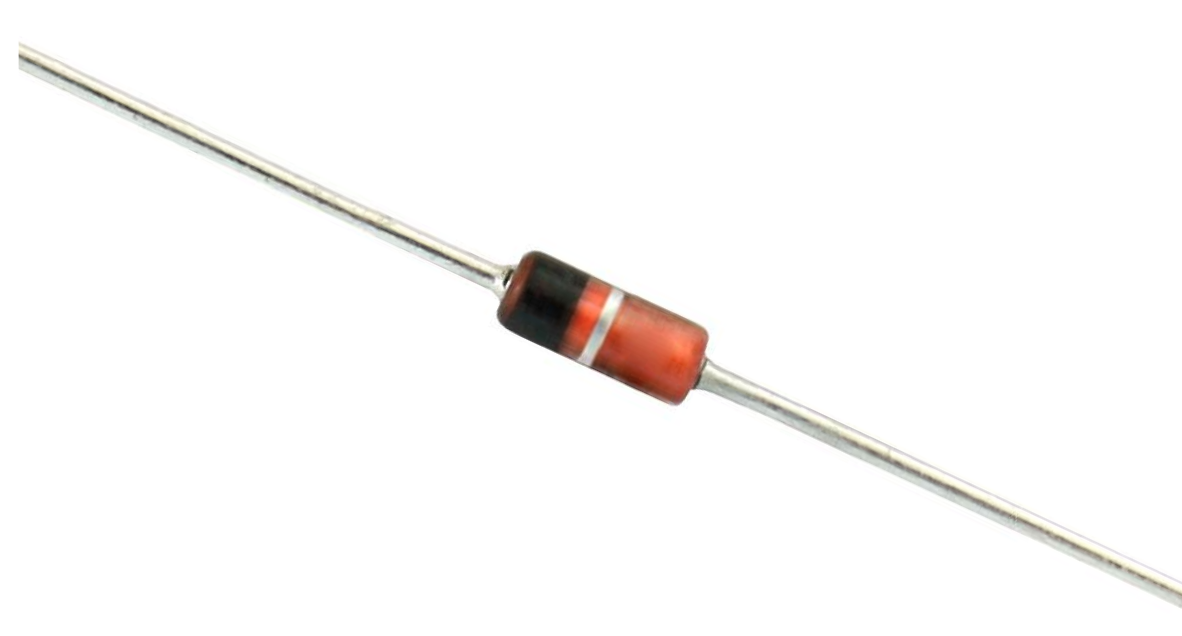
\includegraphics[width=.5\textwidth]{zener.png}}
\caption{Our zener diode}
\end{figure}

The zener diode was given proper voltages to work in reverse bias, specifically in the breakdown region. The overall circuit was identical to that of voltage regulator by zener diode. We gave particularly 5.0 V, 5.5V in two different runs from the powersource. The Zener diode regulated around 4.9 V. 

\begin{figure}[hbt!]
\centering{\centering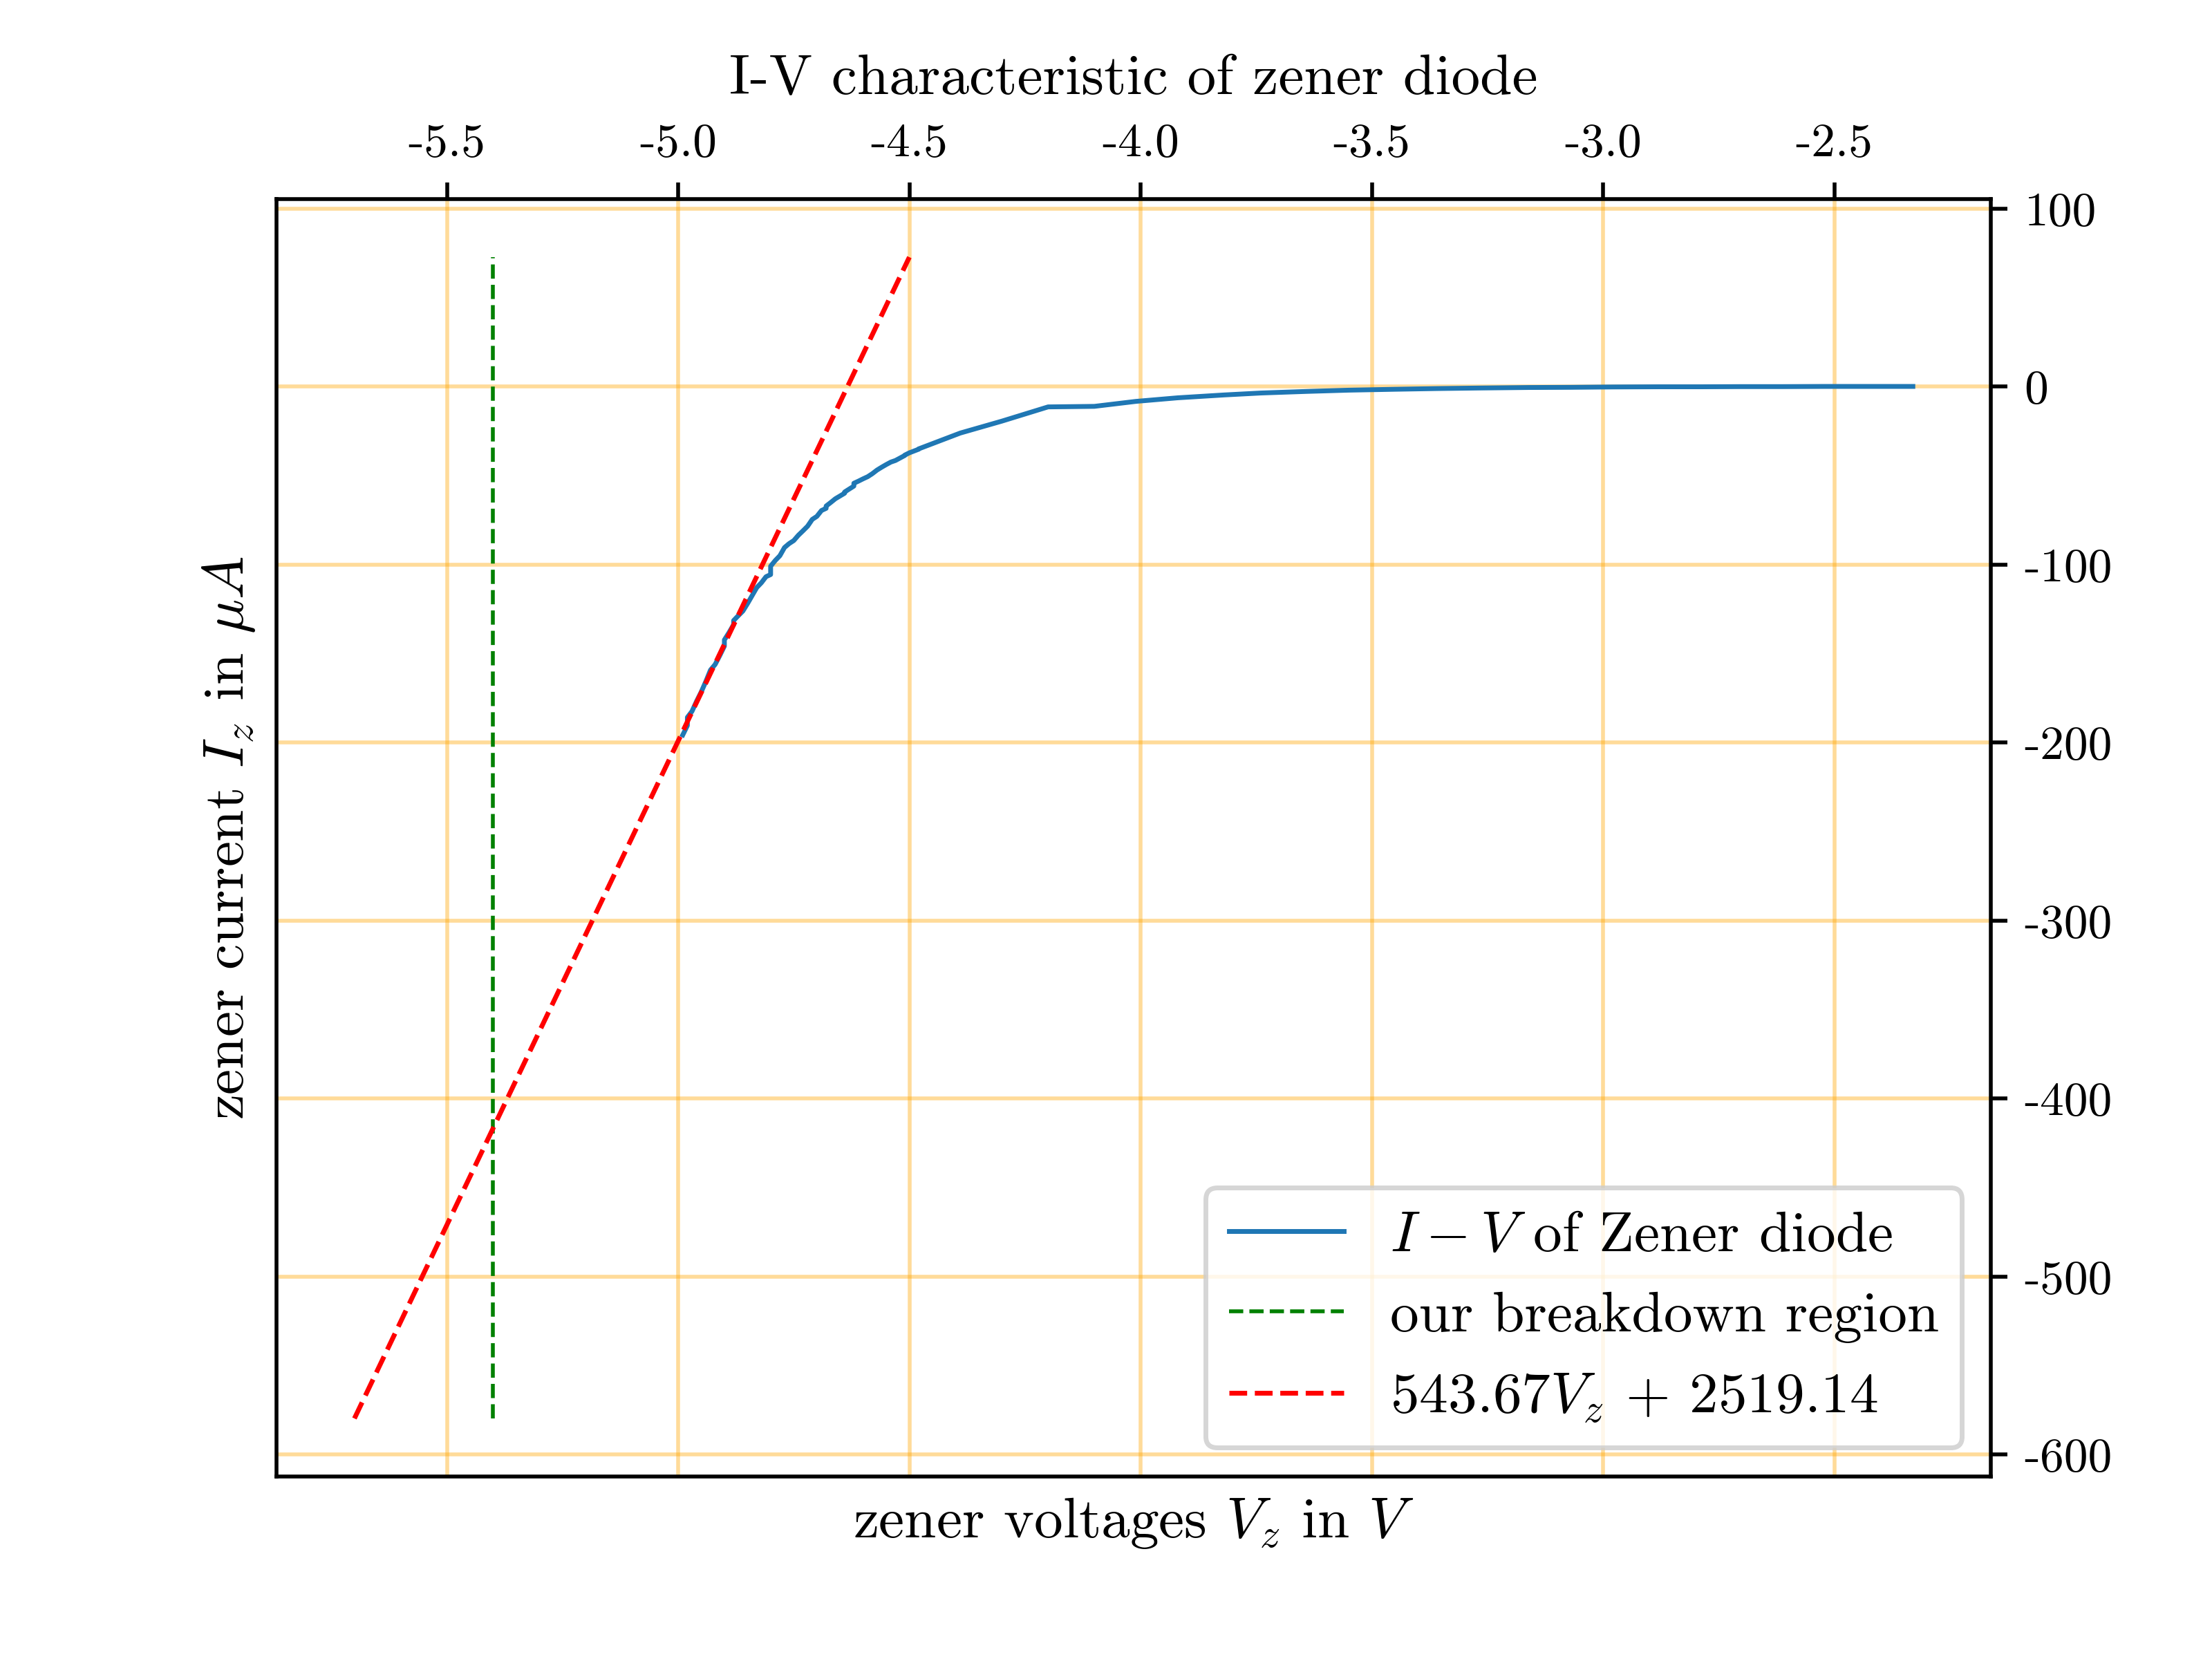
\includegraphics[width=.5\textwidth]{zenerIV.png}}
\caption{current and voltage characterists of zener diode \label{exiv}}
\end{figure}

Now, what we need is that fluctuation over the regulated DC voltage. These fluctuations have to be some function in the frequency domain as we assumed. This function must be made of different harmonics of sinusoidal waves with different phases and frequencies as thought by Fourier and his analysis. So basically we needed a system to measure different amplitudes of these harmonics at different frequencies to model our fluctuations. We needed a complete frequency spectrum at the particular bandwidth we are looking for in this analysis. The LOCK IN amplifier gives exactly that. 


** Measuring instrument: LOCK IN amplifier 

LOCK IN amplifiers came in the 1930s and became very important in signal extraction from given frequency and phase. It is very helpful in measuring signals in a very noisy environment. It takes two inputs, one which is being measured and one which is given as a reference mono frequency signal. Reference signal gets multiplied with input signal and gives output through a process called Phase sensitive detection in which it uses homodyne detection scheme and filters out signal as DC component. We will see in a bit.

*** Phase sensitive detection

In nutshell it uses frequency multiplication and generates double side bands which then pass through a low pass filter to extract signal. In figure \ref{psd} you can see a signal first goes into a low noise differential amplifier which strengthens the signal. Signal Gets multiplied by another reference signal. This gives rise to two bands which pass through a low pass filter which cancels higher degree signal and only left is low frequency signal. 

If we take signal $V_s(t)$ with frequency $w_s$, amplitude $A$ and phase $\theta$. 

\begin{align*}
V_{s} & = A \cos(w_st+\theta)\\
\\
& = \frac{A}{2} (e^{i(w_st+\theta)}+e^{-i(w_st+\theta)}\\
\end{align*}

Reference signal can be taken as following,

\begin{align*}
 = B (e^{-i(w_rt+\phi)})
\end{align*}

In common settings, $\phi = 0$ and $B=1$,

\begin{align*}
 = B (e^{i(-w_rt)}}
\end{align*}

Together after mixing the signals we have,

\begin{align*}
Z(t) & = V_s(t)\timesV_r(t)\\
\\
& = \frac{A}{2}(e^{i\left[ (w_s-w_r)t+\theta \right]}+e^{-i\left[ (w_s+w_r)t+\theta \right]})\\
\\
& = X(t)+Y(t)
\end{align*}

Making $w_s=w_r$ which makes subtraction vanishes and only one term with higher frequency lefts. Passing this signal through a low pass filter with very low cutoff gives only DC components and rejects noise even from neighbouring frequencies.


\begin{align*}
Z(t) & = \frac{A}{2}(e^{i \theta})
\end{align*}

Two component $X(t)$ and $Y(t)$ becomes,

\begin{align*}
X(t) & =Re(Z(t))\\
\\
& =  \frac{A}{2}\cos(\theta)
\end{align*}

And,

\begin{align*}
Y(t) & = Im(Z(t))\\
\\
& =  \frac{A}{2}\sin(\theta)
\end{align*}

So, Amplitude and Phase becomes, 

\begin{align*}
R & = \sqrt{X(t)^2+Y(t)^2}\\
\\
& =  \sqrt{(\frac{A}{2}\cos(\theta))^2+(\frac{A}{2}\sin(\theta))^2}
\end{align*}

\begin{align*}
\Theta & = \arctan(\frac{Y}{X})
\end{align*}

So, the final product in PSD is the absolute amplitude of the signal and its phase. 

*** TIME constant 

*** ENBW

*** sensitivity 

*** sampling rate

*** dynamic reserve

*** LOCK IN amplifier over traditional measuring device/system 

For noise analysis LOCK IN amplifiers are the optimal choice. Traditional approaches deal with the first measurement of a small signal in the time domain. This signal gets amplified with additional noise from the amplifier. Also, amplifiers attenuates signals with its limited bandwidth which is a measure of concern for certain use case scenarios. This attenuated signal gets into some detector. For signal analysis, this signal must go into other  processes like analog to digital conversion then Fourier transformation. This whole process gives too much concerned noise which is not related to devices being analysed in our case the voltage regulator circuit. Alternative approach is to go with a LOCK IN amplifier. Which cancels out most burdens of traditional measurement steps. This whole combined help in reducing internal noise and increasing S/N ratio.

Pros of LOCK IN amplifier: 

LOCK In amplifiers reduces attenuation of signal with increasing frequency since it does not measure signal in the whole frequency spectrum.
Increase S/N ratio over traditional amplifier circuit
Gives direct data into frequency domain

Cons of LOCK IN amplifier:

Relatively expensive
Does not give information in time domain
Relatively slow for whole analysis of frequency domain (low but accurate resolution of frequency domain)


*** SR830 

We used a LOCK IN amplifier from Stanford Research Systems. It is used to detect low amplitude signals as low as $10\frac{nV}{Hz}$ and frequency as low as $100mV$.  and measure very small AC signals -upto few nanovolts. Accurate measurements may be made even when the small signal is obscured by noise sources many thousands of times larger.
Lock-in amplifiers use a technique known as
phase-sensitive detection to single out the component of the signal at a specific reference frequency and phase. Noise signals at frequencies other than the reference frequency are rejected and do not affect the measurements.


Now , on the basis of frequencies/ frequency levels and its origin, there are different types of noises are present in our environment. Some of them are discussed below:


* Methodology

the I-V characteristic of the zener diode and its datasheet which the reader can go through in the appendix. 



** method of data filtering and analysis



What is Lock- in amplifier? and its application in our project


What is phase-sensitive detection?

Lock-in measurements require a frequency reference. Typically an experiment is excited at a fixed frequency (from an oscillator or function generator) and the lock-in detects the response from the experiment at the reference frequency. 
(Figure…. )

In our project we have used the lock-in amplifier to measure the root mean values of different noise voltages( Vrms) at different frequencies. So, in general this instrument detects the phase and frequency of our input signal and compare its phase and frequency with the phase and frequency of our reference signal.If the phase and frequency of both the signals are same then we get Vrms values for different frequencies.If the phase of our reference and input signal are not found to be same then , we cannot able to get the output noise voltages (Vrms).Here in our project, we have used SR830 lock-in amplifier.

The SR830 amplifies the signal and then multiplies it by the lock-in reference using a phase-sensitive detector or multiplier. The output of the PSD issimply the product of two sine waves.

Vpsd = VsigVLsin(ωrt + θsig)sin(ωLt + θref)
= 1/2 VsigVLcos([ωr - ωL]t + θsig - θref) -
1/2 VsigVLcos([ωr + ωL]t + θsig + θref)

The PSD output is two AC signals, one at the difference frequency (ωr - ωL) and the other at the sum frequency (ωr + ωL). 
If the PSD output is passed through a low pass filter, the AC signals are removed. What will be left? In the general case, nothing. However, if ωr equals ωL, the difference frequency component will be a DC signal. In this case, the filtered PSD output will be
Vpsd = 1/2 VsigVLcos(θsig - θref).

Where does the 
lock-in reference come from?

We need to make the lock-in reference the same as the signal frequency, i.e. ωr = ωL. Not only do the frequencies have to be the same, the phase between the signals can not change with time, otherwise cos(θsig - θref) will change and Vpsd will not be a DC signal. In other words, the lock-in reference needs to be phase-locked to the signal reference. 
Lock-in amplifiers use a phase-locked-loop (PLL) to generate the reference signal. An external reference signal (in this case, the reference square wave) is provided to the lock-in. The PLL in the lock-in locks the internal reference oscillator to this external reference, resulting in a reference sine wave at ωr with a fixed phase shift of θref. Sincethe PLL actively tracks the external reference, changes in the external reference frequency do not affect the measurement.

What does the SR830 measure? 

The SR830 multiplies the signal by a pure sine wave at the reference frequency. All components of the input signal are multiplied by the reference simultaneously. Mathematically speaking, sine waves of differing frequencies are orthogonal, i.e. the average of the product of two sine waves is zero unless the frequencies are EXACTLY the same. In the SR830, the product of this multiplication yields a DC output signal proportional to the component of the signal whose frequency is exactly locked to the reference frequency. The low pass filter which follows the multiplier provides the averaging which removes the products of the reference with components at all other frequencies.

RMS or Peak?

Lock-in amplifiers as a general rule display the input signal in Volts RMS. When the SR830 displays a magnitude of 1V (rms), the component of the input signal at the reference frequency is a sine wave with an amplitude of 1 Vrms or 2.8 V pk-pk.

THE FUNCTIONAL SR830

The functional block diagram of the SR830 DSP Lock-In Amplifier is shown below. The functions in the gray area are handled by the digital signal processor (DSP). We'll discuss the DSP aspects of the SR830 as they come up in each functional block description.
(Draw figure….)

THE PHASE SENSITIVE DETECTORS (PSD's)

The SR830 multiplies the signal with the reference sine waves digitally. The amplified signal is converted to digital form using a 16 bit A/D converter sampling at 256 kHz. The A/D converter is preceded by a 102 kHz anti-aliasing filter to prevent higher frequency inputs from aliasing below 102 kHz. The signal amplifier and filters will be discussed later.

This input data stream is multiplied, a point at a time, with the computed reference sine
waves described previously. Every 4 µs, the input signal is sampled and the result is multiplied by the two reference sine waves (90° apart).

The phase sensitive detectors (PSD's) in the
SR830 act as linear multipliers, that is, they multiply the signal with a reference sine wave. Analog PSD's (both square wave and linear) have many problems associated with them. The main problems are harmonic rejection, output offsets, limited dynamic reserve and gain error.

The overall performance of a lock-in amplifier is largely determined by the performance of its phase sensitive detectors. In virtually all respects, the digital PSD outperforms its analog counterparts. 

TIME CONSTANTS and DC GAIN

Remember, the output of the PSD contains many signals. Most of the output signals have frequencies which are either the sum or difference between an input signal frequency and the reference frequency. Only the component of the input signal whose frequency is exactly equal to the reference frequency will result in a DC output.

The low pass filter at the PSD output removes all of the unwanted AC signals, both the 2F (sum of the signal and the reference) and the noise components. This filter is what makes the lock-in such a narrow band detector.

Lock-in amplifiers have traditionally set the low pass filter bandwidth by setting the time constant.The time constant is simply 1/2πf where f is the -3 dB frequency of the filter. The low pass filters are simple 6 dB/oct roll off, RC type filters. A 1 second time constant referred to a filter whose -3 dB point occurred at 0.16 Hz and rolled off at 6 dB/oct beyond 0.16 Hz. Typically, there are two successive filters so that the overall filter can roll off at either 6 dB or 12 dB per octave. The time constant referred to the -3 dB point of each filter alone (not the combined filter).

How big is the DC output from the PSD? It
depends on the dynamic reserve. With 60 dB of dynamic reserve, a noise signal can be 1000 times (60 dB) greater than a full scale signal. At the PSD, the noise can not exceed the PSD's input range. In an analog lock-in, the PSD input range might be 5V. With 60 dB of dynamic reserve, the signal will be only 5 mV at the PSD input. The PSD typically has no gain so the DC output from the PSD will only be a few millivolts! Even if the PSD had no DC output errors, amplifying this milli-volt signal up to 10 V is error prone. The DC output gain needs to be about the same as the dynamic reserve (1000 in this case) to provide a 10 V output for a full scale input signal. An offset as small as 1 mV will appear as 1 V at the output! In fact, the PSD output offset plus the input offset of the DC amplifier needs to be on the order of 10 µV in order to not affect the measurement.

Dynamic reserve in the SR830

The SR830, with its digital phase sensitive detectors, does not suffer from DC output errors caused by large noise signals. The dynamic reserve can be increased to above 100 dB without measurement error. Large noise signals do not cause output errors from the PSD. The large DC gain does not result in increased output drift. 
In fact, the only drawback to using ultra high
dynamic reserves (>60 dB) is the increased output noise due to the noise of the A/D
converter. This increase in output noise is only present when the dynamic reserve is above 60 dB AND set to High Reserve or Normal. However, the Low Noise reserve can be very high as we'll see shortly.

Anti-aliasing filter

After all of the signal filtering and amplification,there is an anti-aliasing filter. This filter is required by the signal digitization process. According to the Nyquist criterion, signals must be sampled at a frequency at least twice the highest signal frequency. In this case, the highest signal frequency is 100 kHz and the sampling frequency is 256 kHz so things are ok. However, no signals above 128 kHz can be allowed to reach the A/D converter. These signals would violate the Nyquist criterion and be undersampled. The result of this under sampling is to make these higher frequency signals appear as lower frequencies in the digital data stream. Thus a signal at 175 kHz would appear below 100 kHz in the digital data stream and be detectable by the digital PSD. 

To avoid this undersampling, the analog signal is filtered to remove any signals above 154 kHz(when sampling at 256 kHz, signals above 154 kHz will appear below 102 kHz). This filter has a flat pass band from DC to 102 kHz so as not to affect measurements in the operating range of the lock-in. The filter rolls off from 102 kHz to 154 kHz and achieves an attenuation above 154 kHz of at least 100 dB. Amplitude variations and phase shifts due to this filter are calibrated out at the factory and do not affect measurements. This filter is transparent to the user.

How does a lock-in measure noise?

Remember that the lock-in detects signals close to the reference frequency. How close? Input signals within the detection bandwidth set by the low pass filter time constant and roll-off appear at the output at a frequency f=fsig-fref. Input noise near fref appears as noise at the output with a bandwidth of DC to the detection bandwidth.

For Gaussian noise, the equivalent noise bandwidth (ENBW) of a low pass filter is the bandwidth of the perfect rectangular filter which passes the same amount of noise as the real filter. The ENBW is determined by the time constant and slope as shown below. Wait time is the time required to reach 99% of its final value.
T= Time Constant

 Slope                 ENBW                Wait Time
6 dB/oct              1/(4T)                       5T

12 dB/oct            1/(8T)                       7T

18 dB/oct            3/(32T)                     9T

24 dB/oct            5/(64T)                     10T

Equivalent Noise Bandwidth ( ENBW )

It is defined as the bandwidth of a perfect rectangular filter that allows the same amount of power to pass as the cumulative bandwidth of the channel selective filters.

Amplifier input noise and Johnson noise of resistors are Gaussian in nature. That is, the amount of noise is proportional to the square root of the bandwidth in which the noise is measured. A single stage RC filter has an equivalent noise bandwidth (ENBW) of 1/4T where T is the time constant (RxC). This means that Gaussian noise at the filter input is filtered with an effective bandwidth equal to the ENBW. In this example, the filter sees 5 µVrms/√Hz of noise at its input. It has an ENBW of 1/(4x100ms) or 2.5 Hz. The voltage noise at the filter output will be 5 µVrms/√Hz x √2.5Hz or 7.9 µVrms.

The amount of noise at the output is determined by the ENBW of the low pass filter.See the discussion of noise later in this section for more information on ENBW. The ENBW depends upon the time constant and filter roll off.

Calculation of ENBW for our data / project work
 
For Sub - 10kHz frequency with time constant (T)= 100 micro-seconds and roll-off =12db/oct :
       ENBW = 1/8T = 1250 Hz 

For Sub - 1Hz frequency with time constant       (T)= 100 milli-second and roll-off =12db/oct :

        ENBW = 1/8T = 1.25 Hz




We have done the noise analysis of noises present in zener diode using lock-in amplifier.
We have obtained the data i.e. the noise voltages (Vrms) corresponding to the different frequencies.With these data we have done the analysis of various noises present in zener diode at various frequencies.


** Interfacing

Results and discussion


We have surveyed voltage regulated circuits we made with zener diodes and found some satisfactory results. We take different results for different bandwidths. For context this is row data from different bandwidth. Here, for each set of frequencies in bandwidth we took almost 50 to 100 readings. 

\begin{enumerate}
\item This is row data for very low frequencies at TIME CONSTANT = $100ms$ and $12db$ \textbf{check unit}\\

[figure]\\

\item This is row data for very low frequencies at TIME CONSTANT = $100ms$ and $12db$ \textbf{check unit}\\

[figure]\\

\item This is row data for very low frequencies at TIME CONSTANT = $100ms$ and $12db$ \textbf{check unit}\\

[figure]

\end{enumerate}




















\addcontentsline{toc}{section}{References}
\bibliographystyle{plain}
\bibliography{documentation}

\end{document}


